\subsection{Tests}

To measure the scalability of Ethereum we prepared some tests to study
the maximal throughput and the size of the blockchain with different
configurations.
To study the scalability of one permission-less blockchain system such as
Ethereum one should prepare some tests using thousand of 
nodes~\cite{bib:securityAndScalabilityPoW, bib:algorand}.
Since we do not dispose of so many resources we take inspiration from
Blockbench~\cite{blockbench}, which compares the performance and scalability
of Hyperledger\footnote{\url{https://www.hyperledger.org/}} and Ethereum in a
\emph{private} scenario, that is when 
we take into consideration a limited number of authenticated nodes.

We tried to use the public available Blockbench 
repository\footnote{\url{https://github.com/ooibc88/blockbench}}
but we did not manage to configure it, because of a lot of hard-coded
configuration variables and the lack of a well-written documentation.
Therefore we desisted and wrote our own system.


\subsubsection{Test Configuration}

To keep the configuration easy we opted for a classic master-slave logic.
The master, i.e. the initiator and coordinator of the tests, uses the ssh
protocol to run commands on the remote machines.
Similarly to~\cite{blockbench} we distinguish the roles \emph{miner} and
\emph{client}. The former is accountable to generate new blocks while the
latter creates and propagates transactions and both roles verify the 
blocks\footnote{To reduce the number of test variables we consider only 
	full nodes}.
We can assign multiple roles to a machine. In this case we run
\emph{one geth instance} for each role.
The coordinator copies the right genesis block in the test machines. 



In each run of test we distinguish at least two phases:
\begin{enumerate*}
	\item the setup, and
	\item the test itself.
\end{enumerate*}


\subsubsection{The Setup}
The setup is used to initialize the different machines with the right genesis
file and the data structures to mine and validate the blocks,  i.e.
the ethash DAG and the ethash cache

\paragraph{Genesis file}

The genesis file contains useful information to create (deterministically)
the genesis block. It contains several parameters, such as the maximum
gas limit for the files, the difficulty and an initial allocation of Ether
for some accounts\footnote{This possibility has been used for the so-called
ICOs (Initial Coin Offering) used by the Ethereum Foundation to obtain fiat
currency to finance the project.}. Each node of the network should be 
initialized with the same genesis file. 
The main network and the official Ethereum test
networks use hard-coded values.

The \textbf{timestamp} of the genesis file, that corresponds to the one of the genesis
block, influences the difficulty of the first blocks, and transitively
of all the blocks.
Since, for time constraints, we want to run each test for few minutes and
at the same time keep the difficulty found with the initial tests,
during the setup phase the initiator reads its timestamp and gives it
as parameter to the peers\footnote{Before starting the test all the
peers should be configured, therefore using the timestamp of the coordinator
does not assume fine-grained coordinated clocks.}

As already described in \autoref{}, the \textbf{difficulty} is an adaptive
parameter  that determines how much effort should be invested in the creation
of a new block. In our test we use the same hardware and same operating system 
in all nodes and for all miners (we deliberately used only one thread for 
mining). Therefore to find a suitable start value for the difficulty for the
different configurations we ran a simulation with one, two, four and 8 miners
for 24 hours.
\autoref{fig:start_difficulty_raw} shows how the difficulty changed with
the different number of miners. We can notice that in our homogeneous system
the final values of difficulties have a quasi linear dependency with the number
of miners. For the test we took as initial value the median of the last 100
blocks.
\begin{figure}
	\begin{center}

		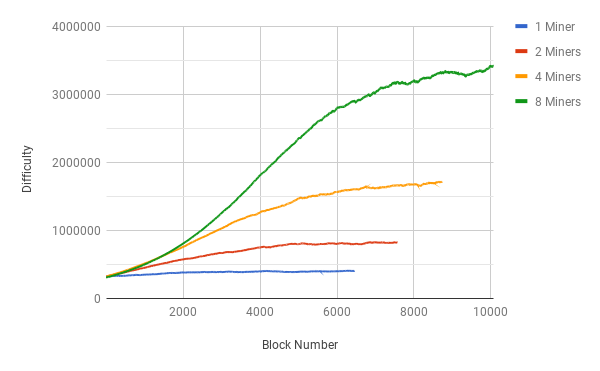
\includegraphics[width=0.8\textwidth]{./res/img/start_difficulty_all.png}
		\caption{The growth of the difficulty in the 24 hour run.}
		\label{fig:start_difficulty_raw}
		
	\end{center}
\end{figure}

\paragraph{Ethash Datastructures} Ethereum uses an improved version of the
Dagger-Hashimoto algorithm, known as 
Ethash~\cite[Appendix J]{wood2018ethereum} as Proof of Work algorithm.
The rationale to use of this memory intensive algorithm is its 
ASIC-resistance. ASIC are specialized hardware used massively in the Bitcoin
ecosystem. These kind of Hardware is a risk for centralization, 
because to begin mining new blocks a big initial investment is needed and
only few entities can afford this cost.

Essentially to create a valid block the miner should find a mixHash and
a nonce (\autoref{fig:world-state}) for the block.
The PoW algorithm takes as input the block without header, the candidate
nonce and a big dataset, known as \textbf{DAG}, and
returns the mixHash and a number $n$. The puzzle is resolved if
$n$ is smaller than $2^{256}$ divided by the difficulty of the block. Clearly,
the higher the difficulty the higher the number of nonce to try to find the
right values. The DAG can be precalcolated and is fixed for each epoch, i.e.
$30000$ blocks, that corresponds roughly to $100$ hours. To verify
that the mixHash and the nonce are correct values only a cache for the
DAG is needed. Actually, the cache is required to generate the DAG itself.
At each epoch the DAG and the cache change and their size increase of
$80$ mebibytes and $128$ kibibytes, respectively.
We refer to the yellow paper~\cite[Appendix J]{wood2018ethereum} to get more
more details on how these data structures are computed.
During the setup phase the nodes with the roles miner generate the 
DAG and the cache for the first two epochs~\footnote{}.





